\subsection{SPARK}

\textit{Apache Spark} is an open source framework developed in the AMPLab at the University of California, campus Berkeley\cite{SparkResearch}. It is a fast and general engine for large-scale data processing, as they describe it themselves. The original goal was to design a new programming model that supports a wider class of applications than MapReduce and at the same time keeping the fault tolerance property of it. They claim MapReduce is inefficient for applications that require a multi-pass implementation and a low latency data sharing across parallel operations, which are common in data analytics nowadays, such as: 

\begin{itemize}
 \item Iterative algorithms: many machine learning and graph algorithms.
 \item Interactive data mining: multiple queries on data loaded into RAM.
 \item Streaming applications: some require an aggregate sate over time.
\end{itemize}

Traditionally, MapReduce and DAG engines are based on an acyclic data flow, which makes them non optimal for these applications listed above. In this flow, data has to be read from a stable storage system, like a distributed file system, and then processed on a series of jobs only to be written back to the stable storage. This process of reading and writing data on each step of the workflow causes a significant rise in computational cost.

The solution proposed offers \textit{resilient distributed datasets (RDDs)} to overcome this issue efficiently. RDDs are stored in memory between queries (no need of replication) and they can rebuild themselves in case of failure as they remember how they were originally built from other datasets by transformations such as \textit{map, group, join}.

\subsection{SPARK streaming}

For this project, Spark streaming plays an important role as it takes a raw data stream and transforms it so that it is possible to process it within the framework. A raw stream of data can come in different forms and through different channels: from a very simple file stream, where whenever a new file is added to a specific location it is recognized as the input, a socket stream where the data comes through the network using a TCP protocol and also integrates with more elaborated sources such as \textit{Kafka, Flume, Twitter, HDFS/S3,} etc.


% \begin{figure}
%  \centering
% \includegraphics[width=2.5in]{streaming-flow1.png}
%  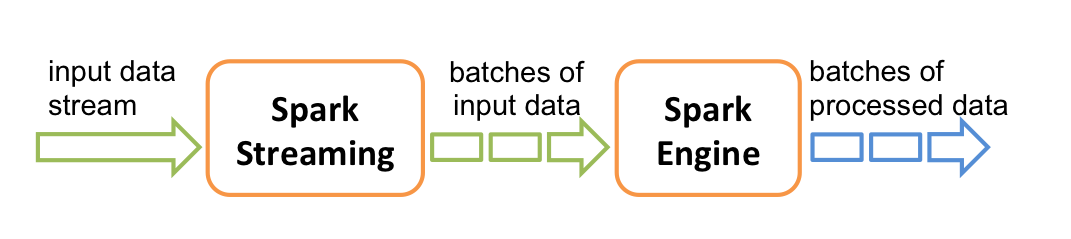
\includegraphics[scale=0.6]{styles/streaming-flow.png}
 % streaming-flow.png: 0x0 pixel, 300dpi, 0.00x0.00 cm, bb=
%  \caption{Flow of data in Spark streaming}
%  \label{fig:streamFlow}
% \end{figure}

\begin{figure}
\centering
% \subfloat[]{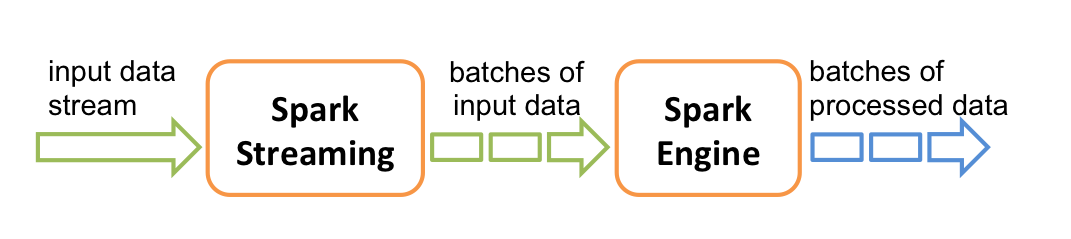
\includegraphics[width=3.1in]{styles/streaming-flow.png}} 
% \subfloat[]{\includegraphics[width=3.1in]{figures/gpgTND.eps}}
\caption{Potential for 0.5 V bias.} 
\label{fig:EcUND} 
\end{figure} 


Figure \ref{fig:streamFlow} shows the general idea of Spark streaming\cite{sparkStreaming}, a raw stream is linked to this module and it converts it to batches of data at user-defined intervals. These batches of data are then treated as RDDs, thus it gets distributed over the cluster where Spark runs. The abstraction of a data stream in Spark is called \textit{DStream}, which stands for Discretized Stream, and is continuous series of RDDs. In a \textit{DStream}, each RDD contains data from a specific interval of time, as it can be seen in Figure \ref{fig:dstream}.


\begin{figure}[h!]
 \centering
 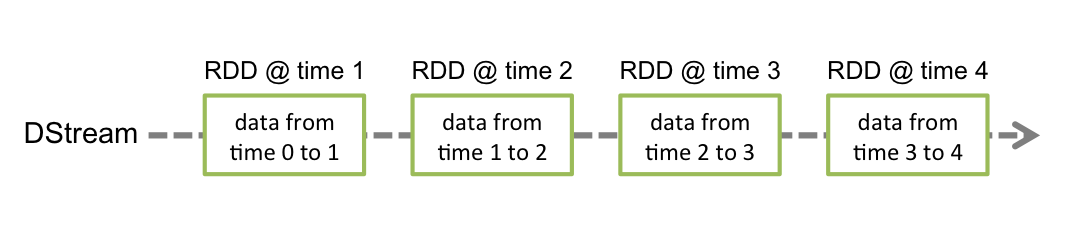
\includegraphics[scale=0.6]{./styles/streaming-dstream.png}
 % streaming-flow.png: 0x0 pixel, 300dpi, 0.00x0.00 cm, bb=
 \caption{DStreams are Spark streaming's abstraction of a data stream}
 \label{fig:dstream}
\end{figure}

\subsection{CluStream}

\textit{CluStream} is a method developed in the Watson Research Center at IBM and the University of Illinois, UIUC. This method presented a different approach on the matter of clustering streams of data with respect to a modified version of \textit{K-Means} which was adapted to work also with data streams. The main difference relies on the separation of the clustering process into two parts: one which would handle the data stream itself gathering only statistically relevant information (online part) and another which actually process the results of the former to produce the actual clusters wanted (offline part). 

Separating the clustering process provides the user several advantages, among others:

\begin{itemize}
 \item by saving only statistical data, rather than the original content, it is possible to save physical storage space (e.g. hard drive space) and therefore reducing costs and allowing a wider range in time to be clustered.
 
 \item The method also allows the analysis of the evolution of the data, as the necessary information for that is contained in the stored statistical information.
 
 \item Because the two parts operate independently it allows the user to select a time horizon, or even a time window, to perform the offline clustering part using the stored statistical information.
\end{itemize}

\subsection{The CluStream framework}

This method is built over a few ideas that need to be conceptualized, which will answer fundamental questions and set up a basis of terminology useful along this work.

\begin{itemize}
 \item \textbf{Micro-Clusters}: that is the given name for the statistical information summaries that is computed during the online component. They are a temporal extension of \textit{cluster feature vectors}\cite{zhang96birch}, which benefit from an additive feature that makes them a natural choice for the data stream problem\cite{clustreamOrig}.
 
 \item \textbf{Pyramidal time frame}: micro-clusters are stored periodically following a pyramidal pattern. This allows a nice tradeoff between the ability to store large amounts of information while giving the user the possible to work with different time horizons without loosing too much precision. The statistical summaries stored are used by the offline component to compute finally the macro-clusters which are the actual clusters the user intended to get.
\end{itemize}

It is assumed that a data stream comes in the form of multi-dimensional records $\bar X_1 ... \bar X_k ...$ where $\bar X_i = (x^1_i ... x^d_i)$.

\begin{definition}\cite{clustreamOrig}

A micro-cluster for a set of d-dimensional points $X_{i_1} ...X_{i_n}$ with time stamps
$T_{i_1} ...T_{i_n}$ is defined as the $2 \cdot d + 3)$ tuple $(\overline{CF2^x},\overline{CF1^x},CF2^t,CF1^t,n)$, wherein $\overline{CF2^x}$ and $\overline{CF1^x}$ each correspond to a vector of d entries. The definition of each of these entries is as follows: 

\begin{itemize}
 \item For each dimension, the sum of the squares of the data values is maintained in $\overline{CF2^x}$. Thus, $\overline{CF2^x}$ contains d values. The p-th entry of $\overline{CF2^x}$ is equal to $\sum^n_{j=1} (x^p_{i_j})^2$. 
 \item For each dimension, the sum of the data values is maintained in $\overline{CF1^x}$. Thus, $\overline{CF1^x}$ contains d values. The p-th entry of $\overline{CF1^x}$ is equal to $\sum^n_{j=1} x^p_{i_j}$.
 \item The sum of the squares of the time stamps $T_{i_1} ...T_{i_n}$ is maintained in $CF2^t$.
 \item The sum of the time stamps $T_{i_1} ...T_{i_n}$ is maintained in $CF1^t$.
 \item The number of data points is maintained in n.
\end{itemize}

\end{definition}

The idea behind the pyramidal time frame is that \textit{snapshots} of the micro-clusters can be stored in an efficient way, such that if $t_c$ is the current clock time and $h$ is the history length, it is still possible to find an accurate approximation of the higher level clusters (macro-clusters) for a user specified time horizon $(t_c - h, t_c)$.

In this time frame, the snapshots are stored at different levels of granularity that depends upon the \textit{recency} of them. These are classified in different orders which can vary from 1 to $log(T)$, where $T$ is the clock time elapsed since the beginning of the stream. The snapshots are maintained as follows:

\begin{itemize}
 \item A snapshot of the $i$-th order occur at time intervals $\alpha^i$, for $\alpha \geq 1$. In other words, a snapshot occurs when $T \bmod \alpha^i = 0$.
 \item At any given moment, only the last $\alpha^l + 1$ snapshot for any given order are stored, where $l \geq 1$ is a modifier which increases the accuracy of the time horizon with the cost of storing more snapshots. This allows redundancy, but from an implementation point of view only one snapshot must be kept.
 \item For a data stream, the maximum number of snapshots stored is $(\alpha^l + 1)\cdot log_{\alpha}(T)$.
 \item For any specified time window $h$, it is possible to find at least one stored snapshot within $2\cdot h$ units of the current time\footnote{The proof can be found in the original article\cite{clustreamOrig}.}.
 \item The time horizon $h$ can be approximated to a factor of $1 + (1/ \alpha^{l-1})$, whose second summand is also referred as the accuracy of the time horizon.
\end{itemize}

\begin{figure}[h!]
 \centering
 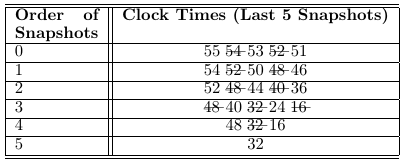
\includegraphics{./styles/pyramidalFrame.png}
 % pyramidalFrame.png: 0x0 pixel, 300dpi, 0.00x0.00 cm, bb=
 \caption{Example of snapshots stored for $\alpha = 2$ and $l=2$}
 \label{table:timeFrame}
\end{figure}

With the help of Figure \ref{table:timeFrame} it is possible to observe how this pyramidal time frame works: snapshots of order 0 occur at odd time units, these need to be retained as are non-redundant; snapshots of order 1 which occur at time units not divisible by 4 are non-redundant and must be retained; in general, all the snapshots of order $i$ which are not divisible by $\alpha^{i+1}$ are non-redundant. Another thing to note is that whenever a new snapshot of a particular order is stored, the oldest one from that order needs to be deleted.

To illustrate the effect on the accuracy of storing more snapshots, the following example is given: supposing that a stream is running for 100 years, with a time granularity of 1 second. The total number of snapshots stored would be $(2^2 + 1)\cdot log_{\alpha}(100*365*24*60*60) \approx 158$ with an accuracy of $1/ 2^{2-1} = 0.5$ or 50\% of a given time horizon $h$. Increasing the modifier $l$ to 10 would yield to $(2^{10} + 1)\cdot log_{\alpha}(100*365*24*60*60) \approx 32343$ maximum snapshots stored with an accuracy of $1/ 2^{10-1} \approx 0.00195$ or $\approx$ 0.2\% which is a significant improvement.


\subsection{Online Micro-clustering}

During this process, the incoming information is analyzed and transformed into statistical summaries that are easier to handle. This process is divided in three parts: initialization, classification and assignation, these are described as follows:

\subsubsection{Initialization}

Before the main maintenance of the micro-clusters, the initialization of $q$ micro-clusters must be performed and each of them are identified with a unique $id$. The number $q$ is taken as a user input and highly depends on the number of final macro-clusters to be calculated and the capabilities of the system where the algorithm runs. 

\begin{itemize}
 \item Random initialization:
 \begin{enumerate}
  \item generate $q$ random d-dimensional vectors to use as centroids of the micro-clusters so that data can be randomly assigned to different micro-clusters. 
  \item Assign the first incoming batch of data to their closest random centroids\footnote{See the assignation process for the details.}.
 \end{enumerate}

 \item KMeans initialization:
 \begin{enumerate}
  \item take the first $n_i$ points, number which is specified by the user, and perform the KMeans clustering method  for $q$ clusters. By doing this it is possible to ensure that the first $n_i$ points will be better clustered than after a random initialization. 
  \item Assign the first incoming batch of data to their closest found centroids.
 \end{enumerate}

\end{itemize}


\subsubsection{Classification}
\label{clus:classification}
When a new batch of data arrives, it is necessary to verify point by point whether they belong to a micro-cluster or not. This means that a point has to be located within a factor $t$ of the RMS deviation\footnote{The RMSD can be obtained using $\overline{CF2^x}$ and $\overline{CF1^x}$ as shown in \ref{findingoutliers}} (RMSD) of the nearest micro-cluster, otherwise it is considered an outlier.

Outliers are taken into account as possible new micro-clusters, this is because the stream of data might change over time. To do so, one new micro-cluster should be created with an entirely new $id$, containing the outlier. The number of micro-clusters $q$ is fixed, so one micro-cluster must be freed either by deleting an old micro-cluster of by merging two of them. To decide whether a micro-cluster is safe to delete, it is necessary to compute its value of \textit{recency} (RV) and compare it to a user defined threshold $\delta$, if no micro-cluster is safe to delete, then the two closest micro-clusters are merged.

\begin{enumerate}
 \item Check if a point $X_{i_k}$ is not an outlier: $distance(\bar X_{i_k}, \hat M_j) \leq t \cdot RMSD$, where $\hat M_j$ is the nearest micro-cluster.
 \begin{itemize}
  \item If $X_{i_k}$ is an outlier: compute $RV_{M_j}$, if $N_j < 2*m$ then the mean the time stamps is used, otherwise compute an approximation for the last $m$ points of each micro-cluster assuming its points are normally distributed\footnote{It is possible to derive the mean and the standard deviation from $CF2^t$ and $CF1^t$ as shown in \ref{handlingoutliers}} for the $1 - m/2N_j$ percentile.
  \begin{enumerate}
   \item If $RV_{M_j} < T - \delta$, where $RV_{M_j}$ is the \textit{recency} value for a given micro-cluster and $T$ the current clock time units elapsed since the beginning of the stream, then $M_j$ is safe to delete and a new micro-cluster $M_{newID}$ must replace it containing $X_{i_k}$.
   \item When there is no $M_j$ safe to delete, then merge $M_j$ and $M_{jj}$ such that $min\{M_j,M_{jj} : M_j,M_{jj} \in M_Q, distance(M_j,M_{jj})\}$, where $M_Q$ is the set of all micro-clusters. The new merged micro-cluster will now have a list of IDs $\{j,jj\}$ and a new micro-cluster $M_{newID}$ must replace $M_{jj}$ containing $X_{i_k}$.
  \end{enumerate}

 \end{itemize}
 \item Assign the point $X_{i_k}$ to $\hat M_j$.

\end{enumerate}


\subsubsection{Assignation}

When a point $X_{i_k}$ is assigned to a micro-cluster, the tuple $(\overline{CF2^x},\overline{CF1^x},CF2^t,CF1^t,n)$ for $M_j$ needs to be maintained, due to its addition properties it is possible to do so directly as follows:

\begin{itemize}
 \item $\overline{CF2^x}_{new} = \overline{CF2^x}_{old} + \overline{CF2^x}_{X_{i_k}} = \overline{CF2^x}_{old}^p + (x^p_{i_k})^2\ \forall p \in \{1,2...d\}$
 \item $\overline{CF1^x}_{new} = \overline{CF1^x}_{old} + \overline{CF1^x}_{X_{i_k}} = \overline{CF2^x}_{old}^p + x^p_{i_k} \ \forall p \in \{1,2...d\}$
 \item $\overline{CF2^t}_{new} = \overline{CF2^t}_{old} + \overline{CF2^t}_{X_{i_k}} = \overline{CF2^x}_{old} + (T_{i_k})^2$
 \item $\overline{CF1^t}_{new} = \overline{CF1^t}_{old} + \overline{CF1^t}_{X_{i_k}} = \overline{CF2^x}_{old} + T_{i_k}$
 \item $n_{new} = n_{old} + 1$
\end{itemize}


\subsection{Offline Macro-Clustering} \label{cluOffline}

While the online process transforms the stream into statistical summaries in the form of micro clusters, the offline process uses this result to deliver the final micro-clusters\footnote{In K-Means this know as the $k$ clusters.} for a given time horizon. This means that the micro clusters in the snapshots stored are now the input data for the macro-clustering process.

Assuming that $t_c$ is the current time and $h$ is the user defined horizon, the time window of information would be $(t_c, t_c - h)$. Having snapshots means that probably $t_c - h$ will not exist in an exact form but the snapshot that occurred just before that time is chosen. The pyramidal time frame ensures that it is always possible to find a snapshot $t_c - h'$ within the user specified tolerance for any $h$.

If $S(t_c - h')$ is the set of micro-clusters at time $t_c - h$ and $S(t_c)$ is the set of micro-clusters at time $t_c$, it is possible to find the final set of micro-clusters $N(t_c,h')$ by subtracting from $S(t_c)$ each corresponding micro-cluster in $S(t_c - h')$. This is possible due to the fact that each micro-cluster is associated with a list of $ids$. Doing this ensures that micro-clusters created before the user specified time horizon do not dominate the the results of the clustering process. 

\begin{property}\label{prop1}
 Let $C_1$ and $C_2$ be two sets of points. Then the cluster feature vector $\overline{CFT(C_1 \cup C_2)}$ is given by of $\overline{CF2(C_1)} + \overline{CF2(C_2)}$
\end{property}

\begin{property}\label{prop2}
 Let $C_1$ and $C_2$ be two sets of points such that $C_1 \supseteq C_2$. Then the cluster feature vector $\overline{CFT(C_1 - C_2)}$ is given by $\overline{CF2(C_1)} - \overline{CF2(C_2)}$
\end{property}

Properties \ref{prop1} and \ref{prop2} show, respectively, the additive and subtractive nature of the cluster feature vectors. This is particularly helpful as only two snapshots are required to approximate any user specified time horizon or window.

Once $N(t_c,h')$ is constructed, the micro-clusters in it are treated as \textit{pseudo-points} K-Means can be used to determine the higher level and final clusters after slightly adjusting it:

\begin{itemize}
 \item At its initialization step, the seeds are sampled with probability proportional to the number of points each micro-cluster has instead of picking them randomly, which correspond to the centroids of the micro-clusters.
 \item The distance from a seed to a \textit{pseudo-point} is equal to the distance between the seed and the centroid of the corresponding micro-cluster.
 \item When the seeds are adjusted, the new seed is defined as the weighted centroid of the micro-clusters in that partition.
\end{itemize}

As a matter of fact, following the previous modifications, many traditional clustering algorithms could be used if needed.
